\documentclass[main.tex]{subfiles}
\begin{document}
\glsresetall

\section{Introduction}

The implementation of the analog L1 Trigger System in the \gls{lst} cameras has been made using a dedicated \gls{asic} \cite{2014ASIC}.\\
The function of the \gls{asic} is to collect the analog signals from the L0 fan-out, add them in three different configurations and discriminate the resulting voltage in order to produce digital trigger output signals.\\
The \gls{asic} was designed to accomplish several specifications needed to ensure the required performance for \gls{cta}: it must be flexible in order to work with the two L0 trigger modes (sum and majority) and to configure the three L1 trigger modes from picture \ref{fig:trigmodes}. The noise must be lower than 0.2 photoelectrons per added channel. The range of the signals processed must be between 0.2 and 100 phe. The gain of the \gls{asic} must be
such that will avoid saturation if the entire signal is concentrated in one channel. Bandwidth must be greater than 500MHz to avoid \gls{nsb} pulses being added with the signals. Because all the electronics are installed inside the camera box, the \gls{asic} must be compact and have a low power consumption $(< 150 mW/ch)$. The scheme of \gls{asic} is shown in picture \ref{fig:l1diagram}.

\begin{figure}[h]
  \centering
  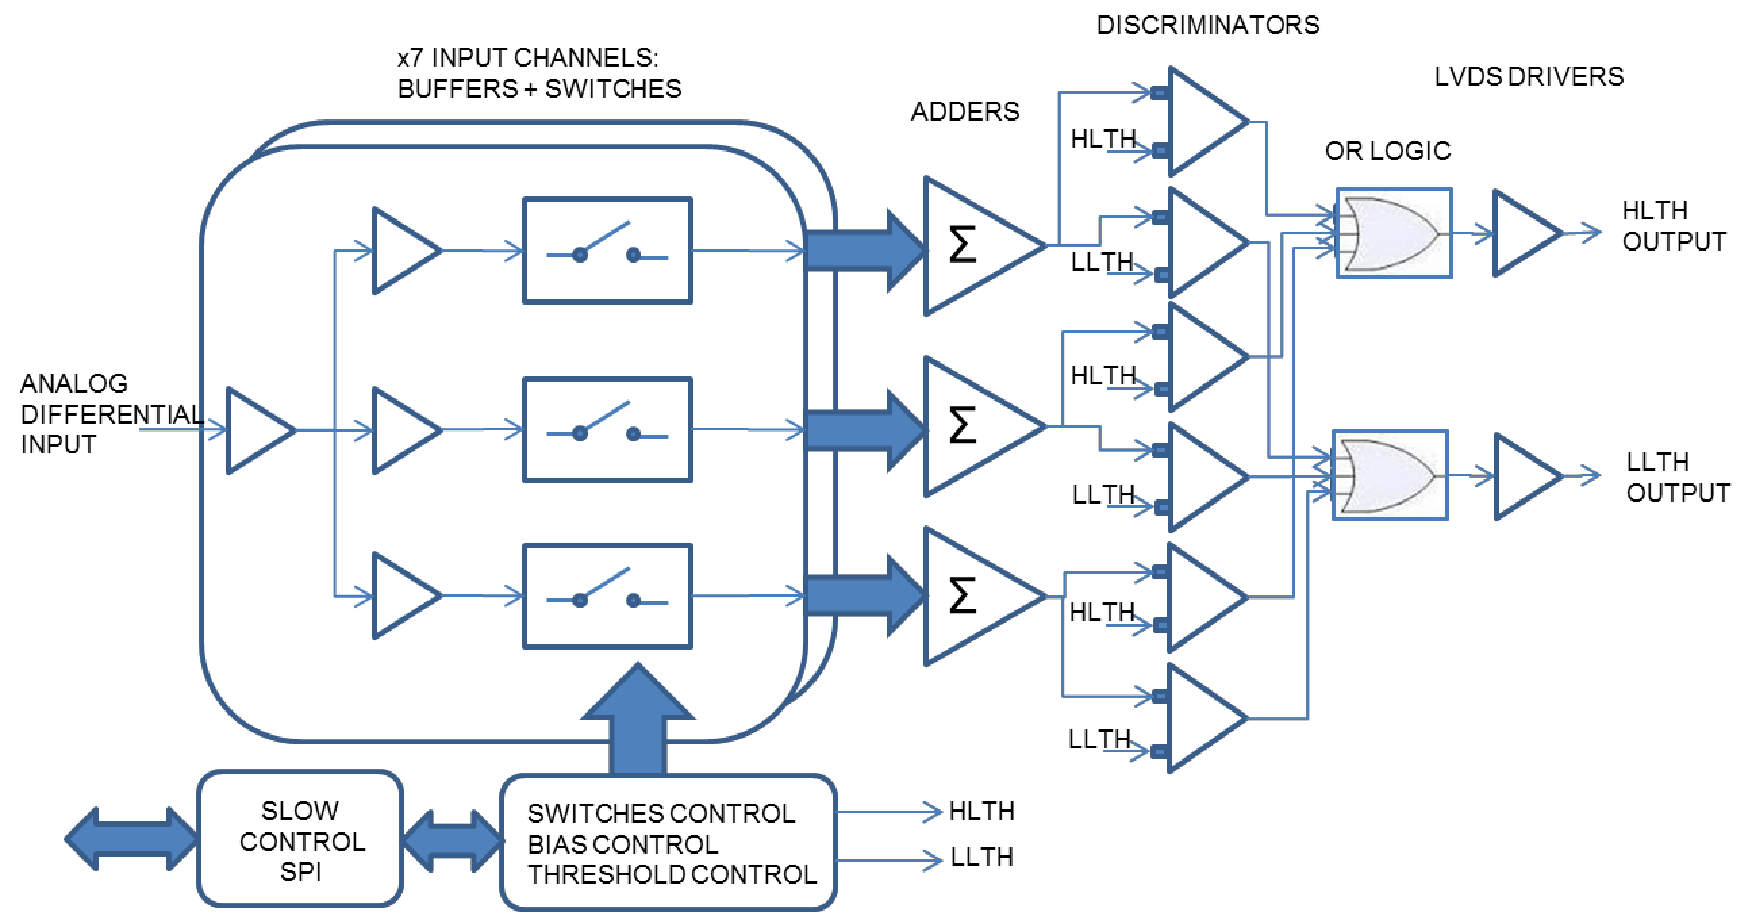
\includegraphics[width=\textwidth]{./Pictures/L1blockdiagram.pdf}
  \caption{L1 \gls{asic} Block diagram}
  \label{fig:l1diagram}
\end{figure}

In the \gls{asic}, there are seven input differential analogue channels and two output differential digital channels. The seven signals arriving to the input channels are replicated three times and sent to three analogue adders (named A, B and C). The signals in each adder are selected by a set of switches, corresponding to the different configurations of the three trigger modes.
The output of the adders is sent to two discriminators, which make the comparison of the added signal with a threshold voltage.
The two discriminators have a different and independent threshold voltage, a low level and high level threshold, generated by differential \glspl{dac}.
The discriminator outputs are connected to two OR gates which are in turn connected to \gls{lvds} transmitters that provide the trigger signal.\\
About ~400 asics where produced at CIEMAT, passing a quality control to validate their performance. The quality control tests probed several characteristics of the \glspl{asic}, such as gain, noise and offset, for all the channels, adders and discriminators. From all the \glspl{asic} tested, 389 surpassed the quality control test and the results where analyzed to characterize the general behaviour of the \gls{asic}. Averaging to all the \gls{asic} analyzed, the result is an overall view of the features that a default \gls{asic} would have, shown in table \ref{tab:allasicsdata}. In this appendix, the results of the characterization of the L1 \glspl{asic} produced at CIEMAT are summarized, using the data from the quality control tests.

\section{Quality control test}

The quality control test consisted of several steps to qualify the behaviour of the \gls{asic} in its different parts (seven input channels, three adders and two \gls{lvds} outputs).\\
The quality control provided a datasheet for each individual \gls{asic} with the results of the tests which where analyzed to charanterize the manufactured \glspl{asic}. Each combination of channel (7), adder (3) and discriminator(2) is accounted separately, having a proper gain, offset and noise. This procedure allows the detection of outliers that could imply the existence of a defect in a part of the \gls{asic}. The quality control tests provided direct measures of offset and noise, but gain must be calculated from the rate scan results in the test voltage. This procedure also offers other way of measuring the offset. The computation of gain and offset from the rate scan, described in section \ref{sec:ratescan}, was perfomed considering a linear behaviour of the input voltage vs. threshold voltage for the 50\% trigger rate. From a linear fit, the gain and offset are obtained. In the next sections, the different steps of the quality control test are described.

\subsection{Test DAC}

Measurement of the maximum and minimum voltage of the \gls{dac} was taken directly from the output pin of the \gls{asic} by a multimeter. Each \gls{dac} set is composed by 2 \glspl{dac} of 9 bits to get a final resolution of 10 bits (positive and negative parts). The measurement is made setting the code in the register with the maximum  and minimum values for both positive and negative parts.

\subsection{Voltage Test: Rate scan} \label{sec:ratescan}

The Voltage test measured the gain of all seven input single channels and the two outputs for 10 different voltages (from 100mV to 1000mV) using a rate scanmethodology, consisting on the comparison of the input trigger rate from a generator on the evaluation setup and the \gls{asic} trigger output rate. This computation is performed with scalers implemented in the FPGA board.

\subsection{Test Adder Channels}

The gain of different sum combinations was obtained by the same rate scan methodology. There are 3 different methods combining different channels of different adders.

\subsection{Analog Offset test}

The Analog offset test consisted in the measurement of the offset in the Analog Adder Output test, which is the output of a multiplexor that selects among the available analog output adder, plus a buffer for the output pins. The measurement is made directly from the differential output pin of the \gls{asic} by a Multimeter.

\subsection{Digital Offset test} \label{sec:digoff}

The Digital offset test procedure measures the offset in the \gls{lvds} digital outputs, by the evaluation of the output status as a funtion of the threshold. The methodology consists in increasing the threshold from 0 Volts using the \gls{dac} values until finding the minimum value where the output goes from 1 to 0, and the maximum for which it goes from 0 to 1. The voltage difference between this two points is the noise of the digital output, and the mean point is the offset. Setting the Threshold to 0, three possible behaviours are observed:
\begin{itemize}
\item If the status of the digital output is a logic '1' (tagged as type 'Pos') it is possible to measure the minimum and the maximum points and therefore it is possible to calculate the offset and the noise.
\item If the status of the digital ouput is a logic '0' (tagged as type 'Neg'), it is not possible to measure neither the minimum nor the maximum point, and then a value of zero is assigned by the program both to the noise and the offset.
\item If the status of the digital ouput is switching (tagged as type 'Com'), it is only possible to measure the maximum value, and the other is assigned to 0. In this case the noise is understimated and the threshold is overstimated.
\end{itemize}

\section{Characterization of the \gls{asic}}

In this section, the results from the quality control tests for all \glspl{asic} are analyzed and discussed.

\subsection{Rate Scan Fit}

For the calculation of the gain, the output of the Voltage test is used to perform a linear fit. If we assume a linear model, the relation between the input voltage and the rate scan result should be:

\begin{equation}
  \label{eq:fit}
  V_{rs} = Gain*V_{input} + Offset
\end{equation}

In figure~\ref{fig:linearfit} the rate scan result versus ten input voltages for a certain path (channel, adder, discriminator) of one \gls{asic} is shown. The linearity can be easily appreciated, specially for low input voltages (under 500 mV).

\begin{figure}
  \centering
  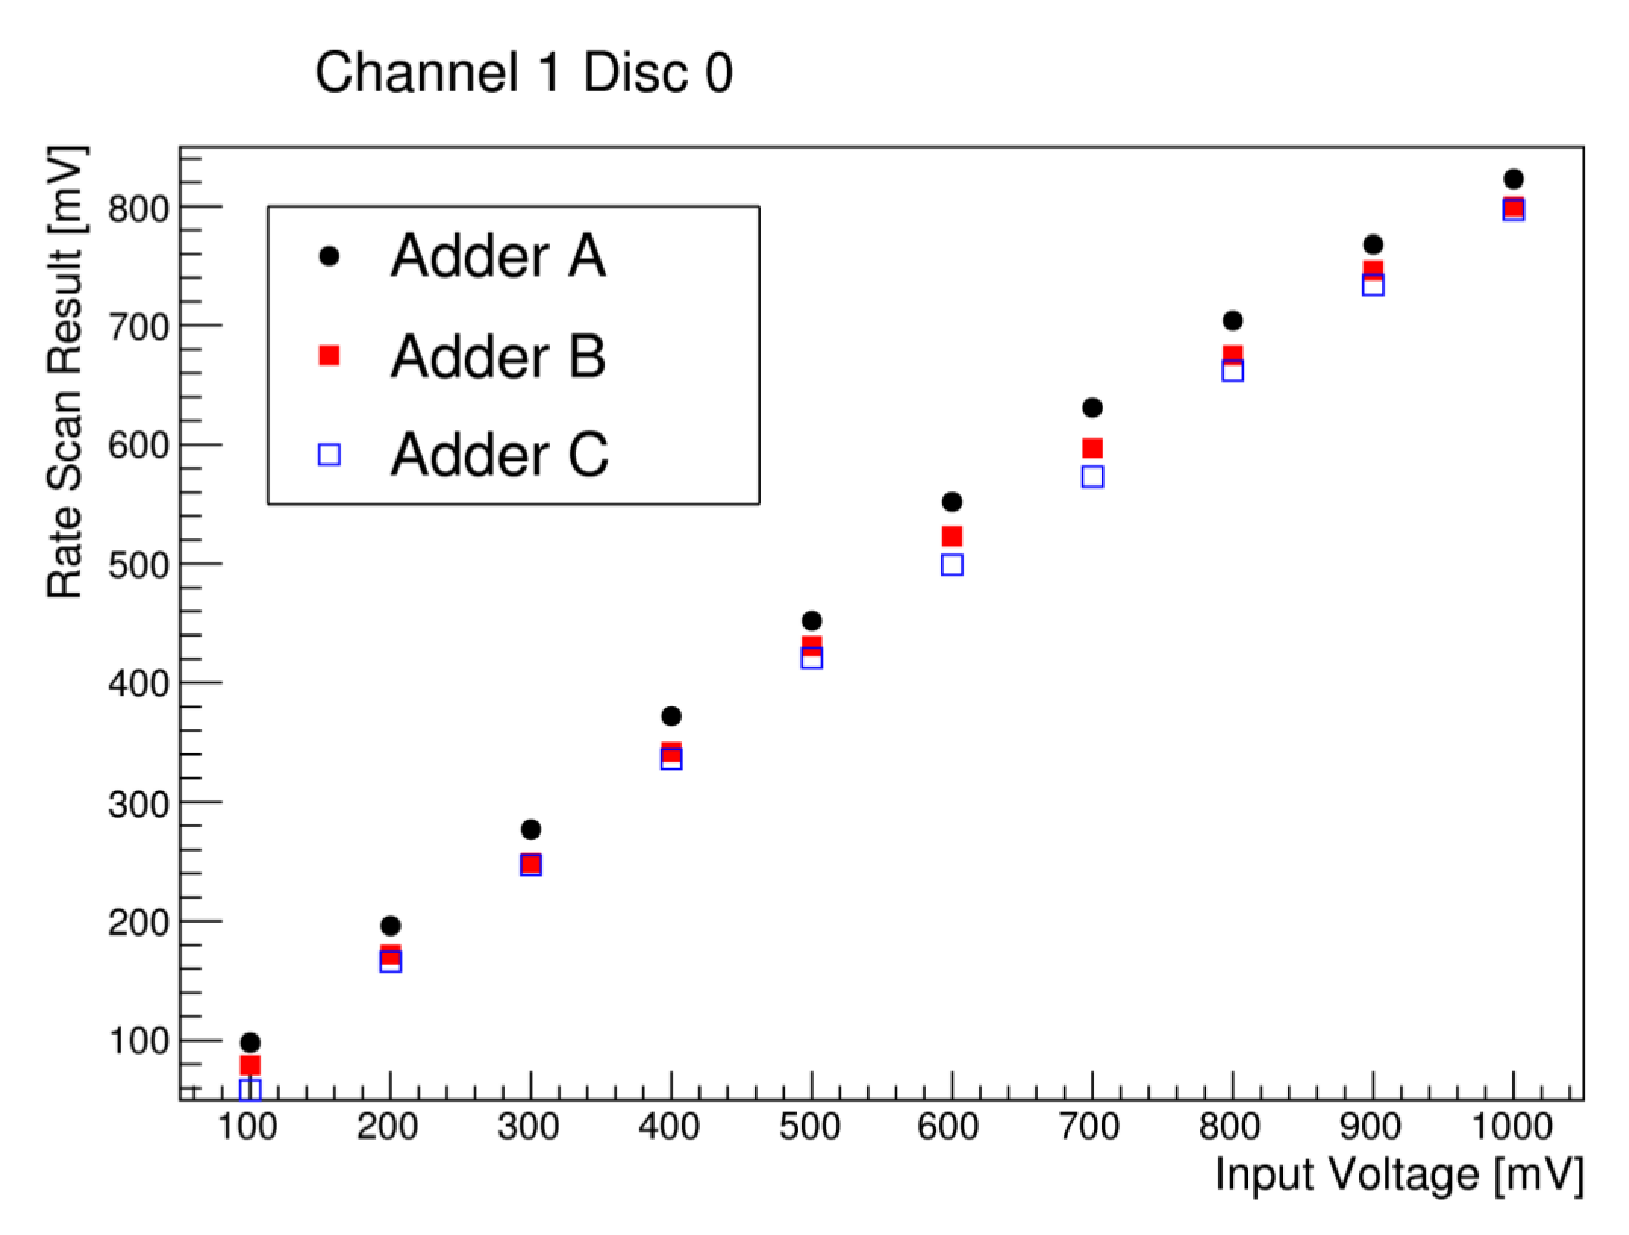
\includegraphics[width=0.6\textwidth]{./Pictures/linearfit.pdf}
  \caption{Rate scan result from one of the voltage tests for \gls{asic} \#61. It can be observed a linear tendency which deteriorates at high voltages.
    Similar plots where obtained from the rest of channel-adder-discriminator combinations. }
  \label{fig:linearfit}
\end{figure}

Where $V_{rs}$ represents the threshold voltage that gives a rate of 50\% trigger, and $V_{input}$ is the input voltage. The use of this method has the advantage of obtaining not only the gain but also the offset of the \gls{asic} without having to measure it with a multimeter. Since linearity seems to depend on the input voltage, it is necessary to consider a range for the fitting where the linearity is better. To do so, several ranges were fitted and the offset obtained was compared to the offset measured with the multimeter in the analog offset test. The range where the difference between the two offsets was lower was selected as the best range to fit the linear model. The resulting range was from 0 V to 300 V and so this range was used to calculate the gain and offset for every path of each \gls{asic}.

\subsection{Gain}

The gain was caclulated with the model fitting decribed in the previous section. Figure~\ref{fig:gaindist} shows the distribution of gain values over the paths of the 389 asics. A clear gaussian profile is observed, centered in the characteristic gain of 0.87, the expected result according to the design specifications. Some outliers were identified having gain values that are too low for the requisites of the \gls{asic}, which could mean a malfunctioning in the \gls{asic}. Fitting the distribution to a gaussian, it is possible to see that the probability of an \gls{asic} to have a gain lower than 0.7 in any of its paths is lower than 0.025\%. There are some outliers with higher gain values, but the probability of any entry to have a gain over 1.05 is lower than 0.007\%. The outliers are identified in image~\ref{fig:gaindist} by their \gls{asic} number.
\\
\begin{figure}
  \centering
  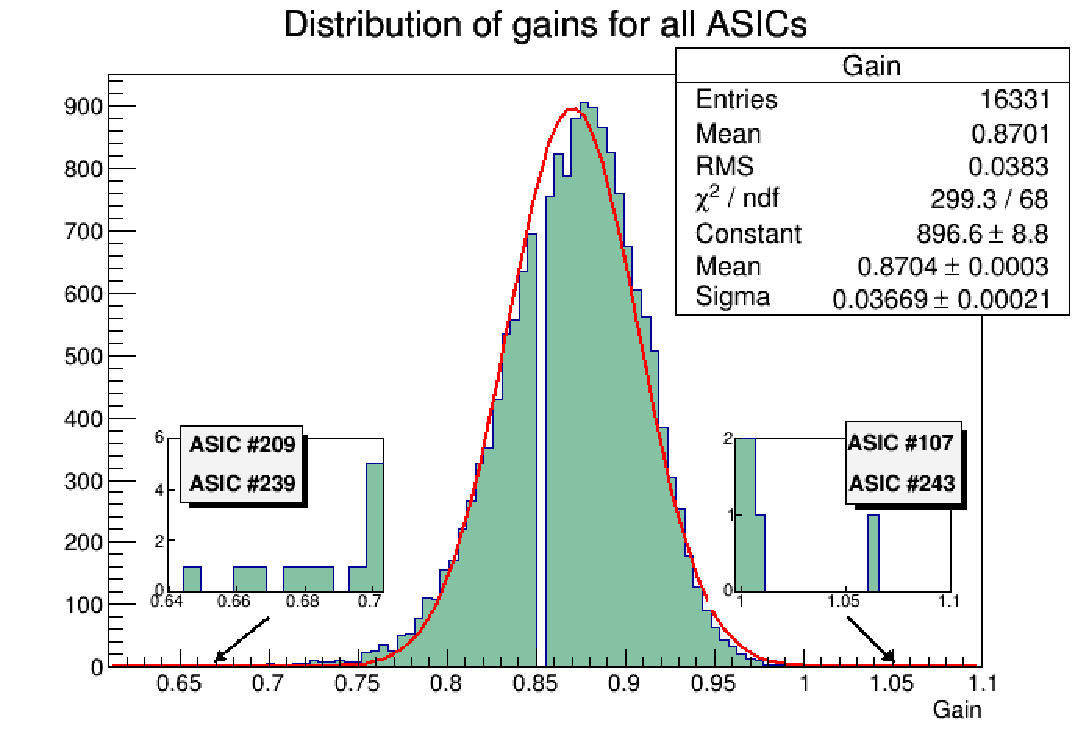
\includegraphics[width=0.8\textwidth]{./Pictures/gaindistribution.pdf}
  \caption{Distribution of gains for all \glspl{asic}. Each entry represents the gain of one possible path (combination of channel-adder-discriminator). The red line represents a gaussian fit with mean 0,8704 and sigma 0,3669.
    The zoom-ins show several outliers with gains very deviated from the average.}
  \label{fig:gaindist}
\end{figure}

Cleaning the outliers from the sample, the characteristic gain is $0.87 \pm 0.038$, obtained from the gaussian fit. This is an average to all the possible paths of channel, adder and discriminator in the \glspl{asic} analyzed. A single path characterization is given in table \ref{tab:allasicsdata}, each entry averaged to all \glspl{asic}.
When obsserving the average gain for each channel separately in table~\ref{tab:gainch}, and in image \ref{fig:gainch} it can be observed that the second channel has a slightly lower gain than the others, and the third one a slightly higher gain. This effect comes out from the configuration used during the quality control tests. The third channel was connected directly to the pulse generator, while the second channel had to be fed with a cable of different length than the others.

\begin{table}
  \centering
  \begin{tabular}{|l|l|l|l|}
    \hline
    Channel & Mean Gain & RMS \\
    \hline
    1 & 0.871 & 0.035 \\
    2 & 0.839 & 0.036 \\
    3 & 0.880 & 0.036 \\
    4 & 0.873 & 0.036 \\
    5 & 0.876 & 0.036 \\
    6 & 0.873 & 0.036 \\
    7 & 0.878 & 0.036 \\
    \hline
  \end{tabular}
  \caption{\label{tab:gainch} Mean gains for the seven channels, averaged to the sample of all asics, without the outliers.}
\end{table}

\begin{figure}[h]
  \centering
  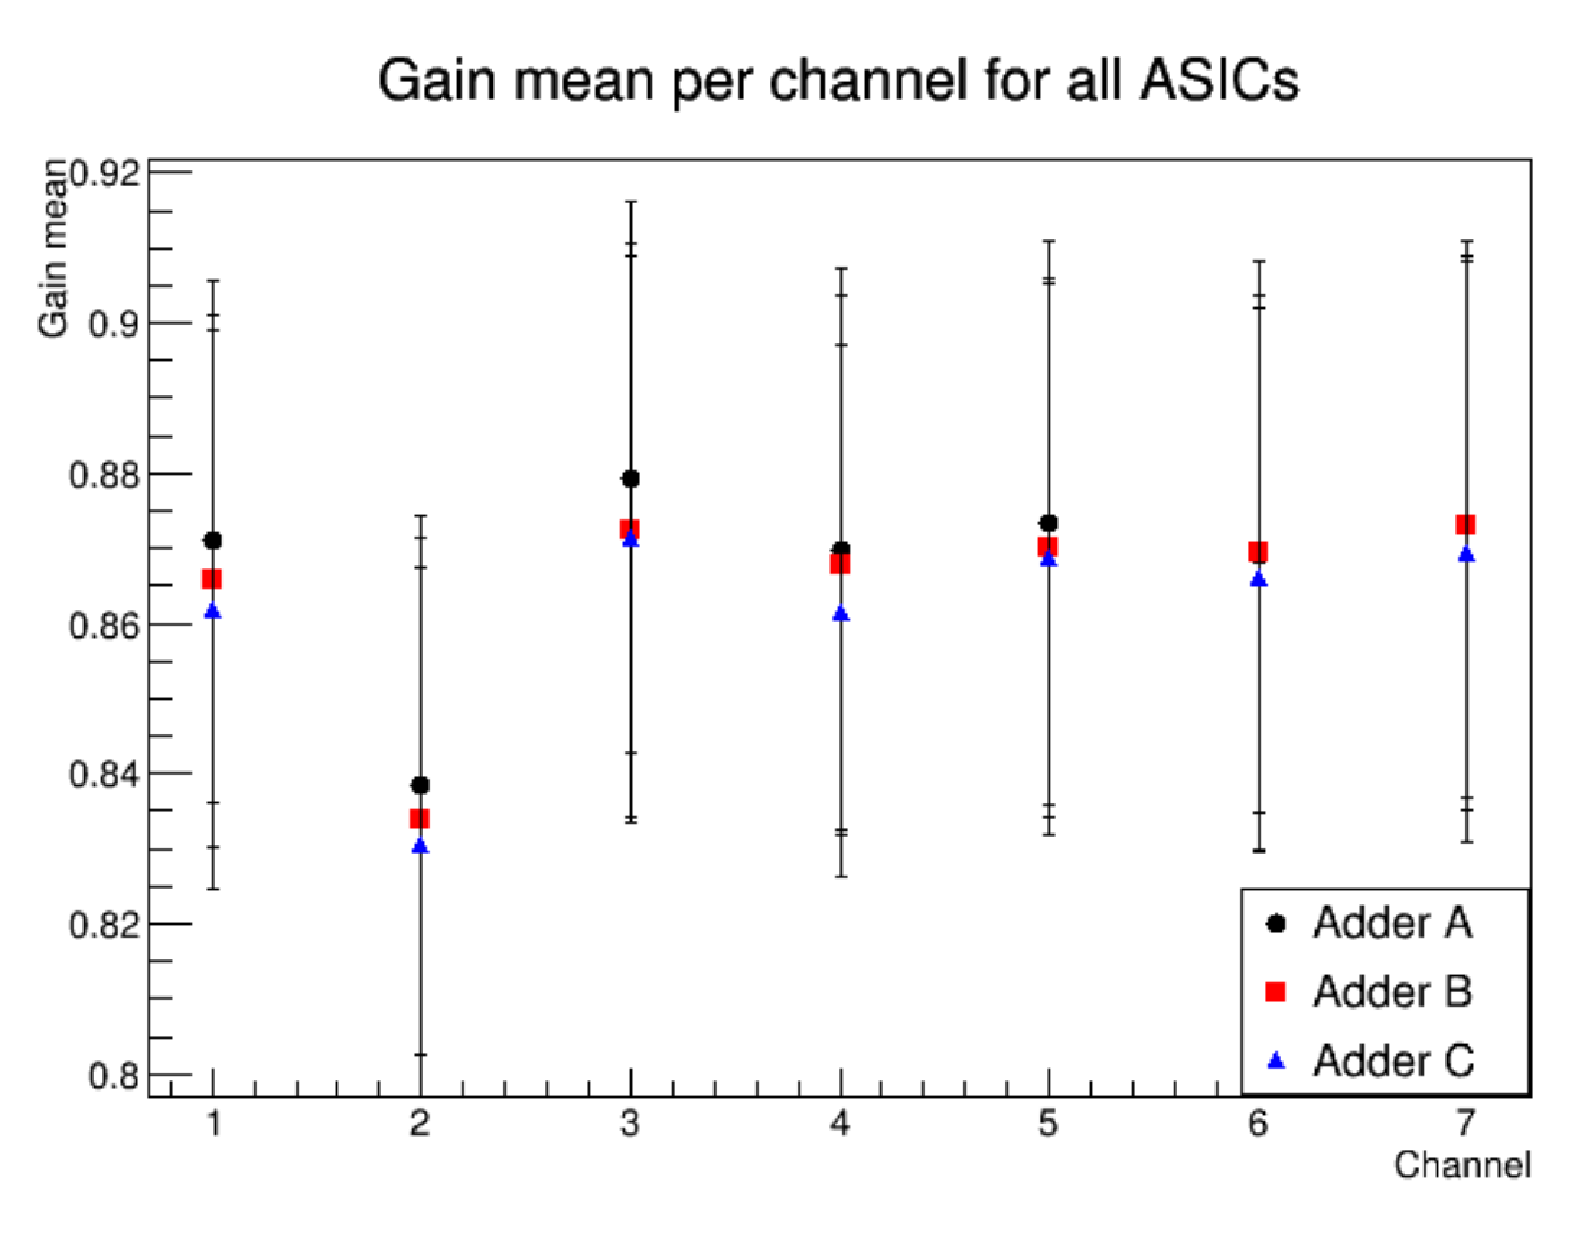
\includegraphics[width=0.7\textwidth]{./Pictures/gainschannel.pdf}
  \caption{Distribution of gains for all \glspl{asic}. Each entry represents the gain of one possible path (combination of channel-adder-discriminator). The red line represents a gaussian fit with mean 0,8704 and sigma 0,3669.
    The zoom-ins show several outliers with gains very deviated from the average. }\label{fig:gainch}
\end{figure}

To find if any part of the \gls{asic} is dominating the fluctuations of the gain, correlation plots between channels, adders and discriminators were studied. A remarkable correlation is not observed in any of the elements of the \gls{asic}, so we can conclude that all parts contribute to the final value of the gain in a similar way. 

\subsection{Offset}

The offset has been measured in three different ways. In the tests, the analog offset was directly measured with a multimeter, the digital offset was measured using the procedure described in section~\ref{sec:digoff},
and finally, from equation~\ref{eq:fit} an offset value that will be called fit offset was calculated.\\
In figure~\ref{fig:offsetdist} the distribution of the analog and digital offsets are shown. It must be noted that it was not possible to measure the digital offset for all the configurations, only the ones with an output status tagged as ``Pos'', so it's not possible to measure negative values of digital offset. Some outliers were detected, with digital offset values very deviated from the mean, which has been removed from the sample at the final characterizaton. Those outiers correspond to \glspl{asic} 110, 209,248 and 437.
\begin{figure}
  \centering
  \minipage{0.5\textwidth}
    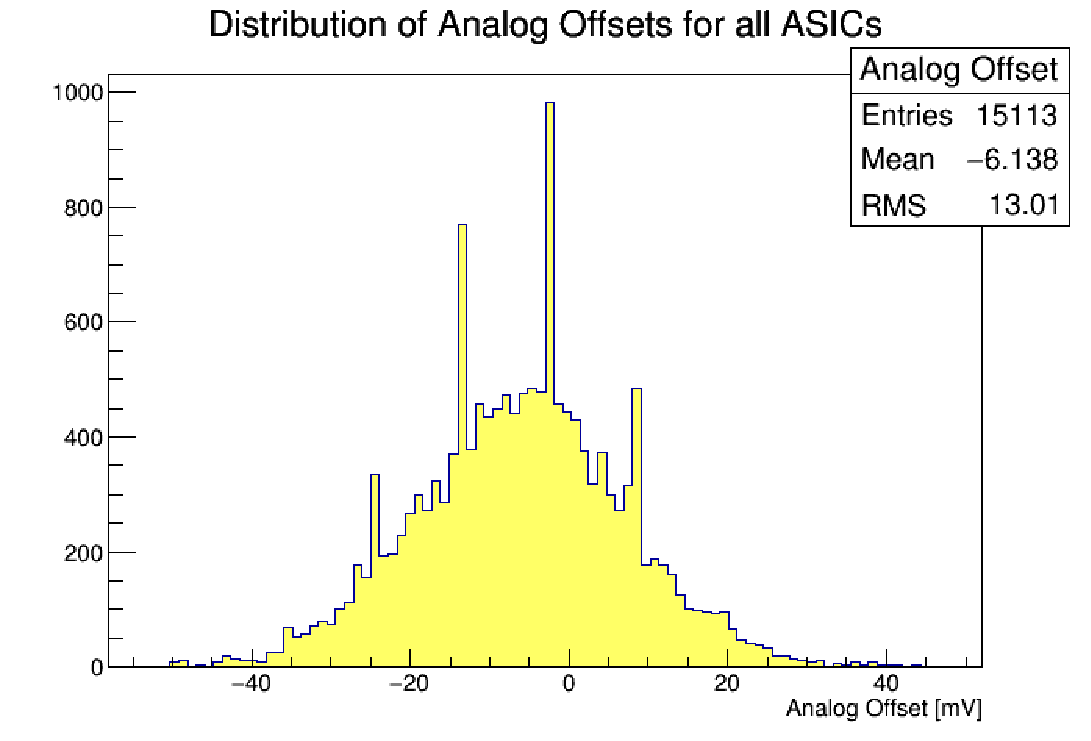
\includegraphics[width=\textwidth]{./Pictures/analogdist.pdf}\\
  \endminipage
  \minipage{0.5\textwidth}
    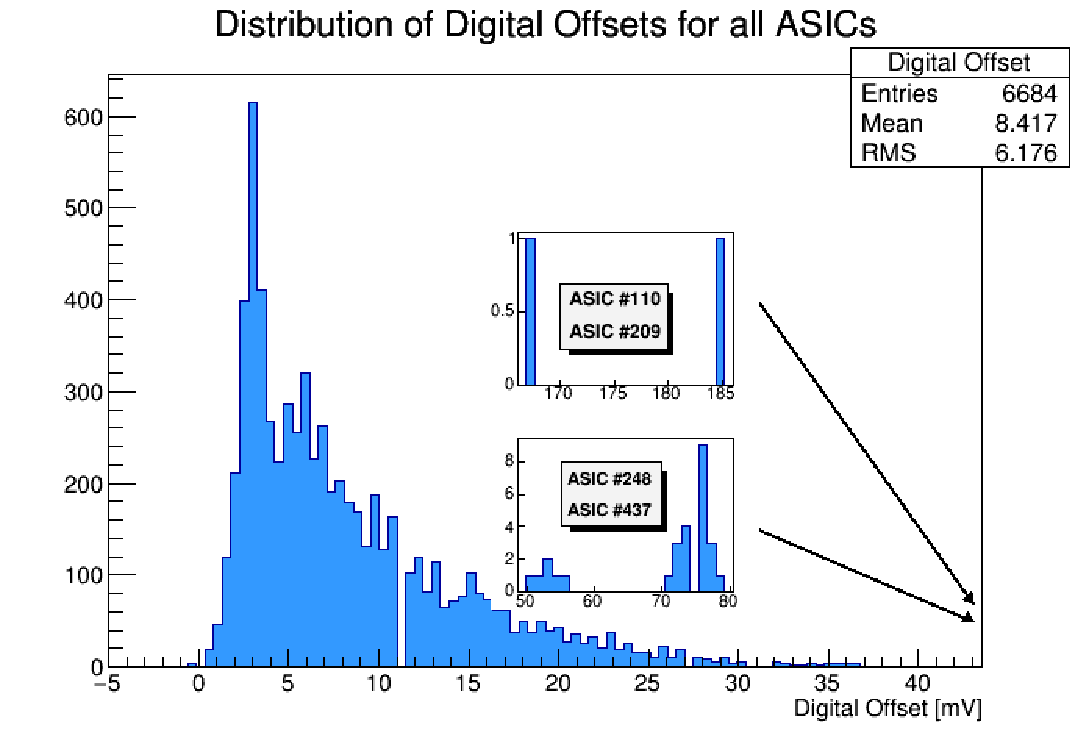
\includegraphics[width=\textwidth]{./Pictures/digitaldist.pdf}
  \endminipage
  \caption{Distribution of offsets for all \glspl{asic}. Each entry represents the offset of one possible path (combination of channel-adder-discriminator).\textit{Top:} Analog offset. \textit{Bottom:} Digital offset. The zoom-ins represent outliers in the digital offset.}
  \label{fig:offsetdist}
\end{figure}

The averaged value of the analog offset is $-6.138 $ mV with RMS of $13.01 $ mV while for the digital offset the mean is $8.41$ mV with RMS of $6.17 $ mV. Plotting the correlation between the two measured offsets(~\ref{fig:offsetcor} it can be seen that there is a correlation between the two ways of measuring the offset.
\begin{figure}
  \centering
  \minipage{0.5\textwidth}
  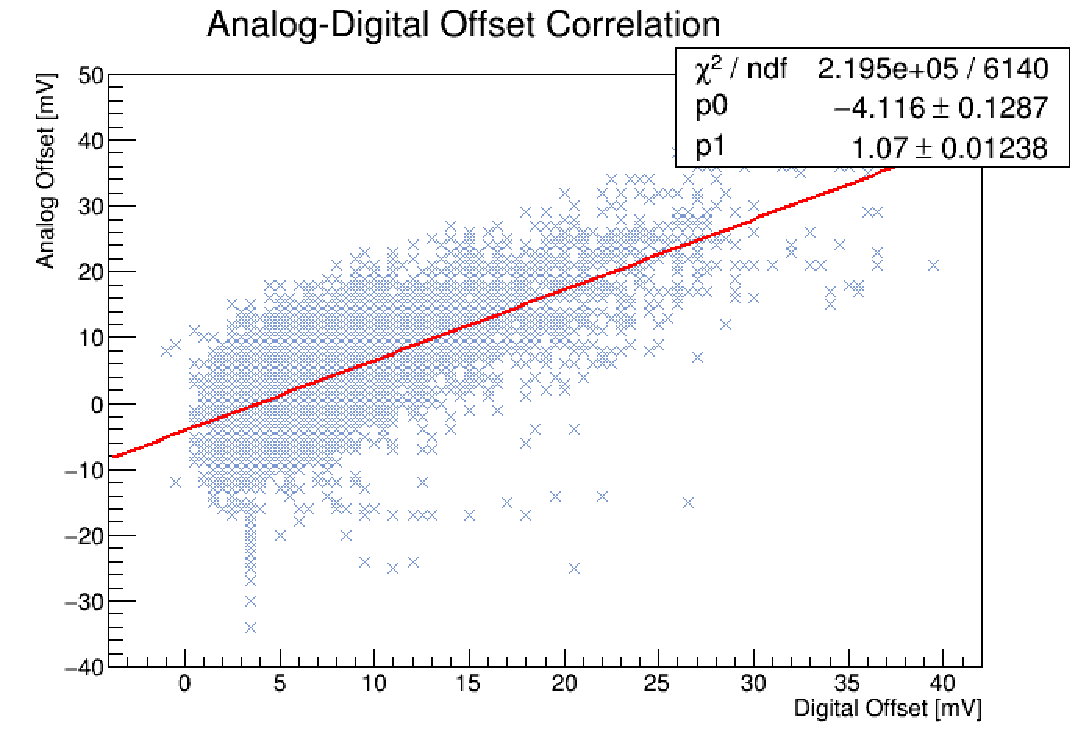
\includegraphics[width=\textwidth]{./Pictures/offsetscor.pdf}
  \endminipage
  \minipage{0.5\textwidth}
  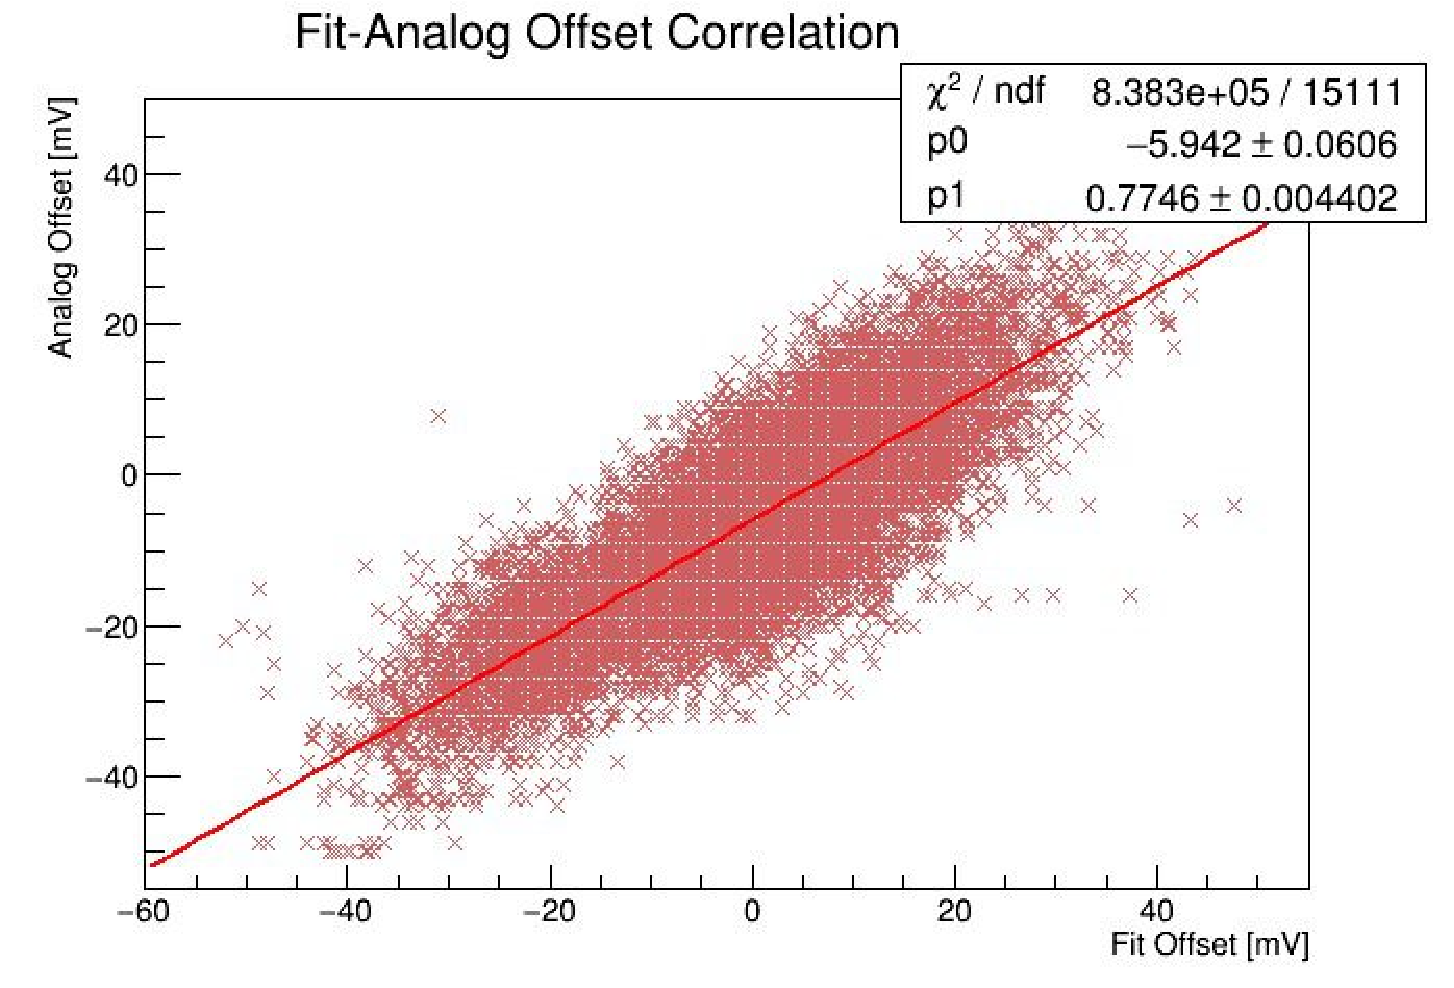
\includegraphics[width=\textwidth]{./Pictures/fitanalogcor.pdf}
  \endminipage
  \caption{\textit{Left}: Correlation between analog offset and digital offset. \textit{Right:}Correlation between analog offset and fit offset.}
  \label{fig:offsetcor}
\end{figure}
Regarding the fit offset, the distribution of the obtained values is shown in figure~\ref{fig:fitoffdist}. To check the validity of this method of obtaining the offset value, the difference between the fit offset and the analog offset has been studied. The averaged value of the fit offset is $0.1334$ mV  with RMS $13.75$ mV. The mean difference between the analog offset and the fit offset is of $5.55$ mV with RMS $8.06$ mV.
\begin{figure}
  \centering
  \minipage{0.5\textwidth}
  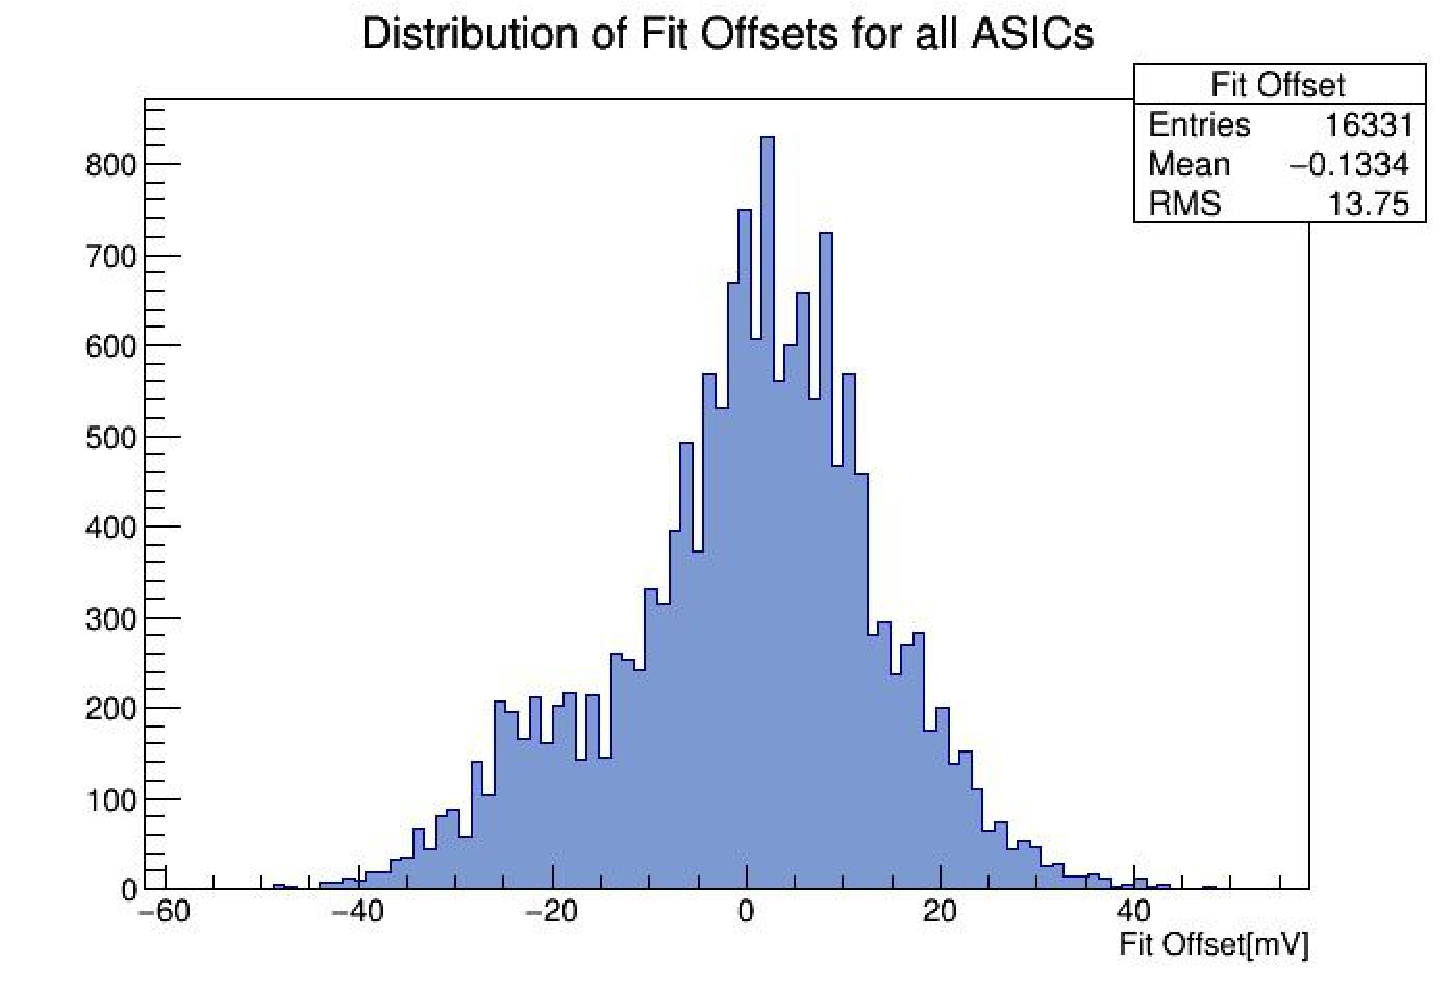
\includegraphics[width=\textwidth]{./Pictures/fitoffsetdist.pdf}
  \endminipage
  \minipage{0.5\textwidth}
  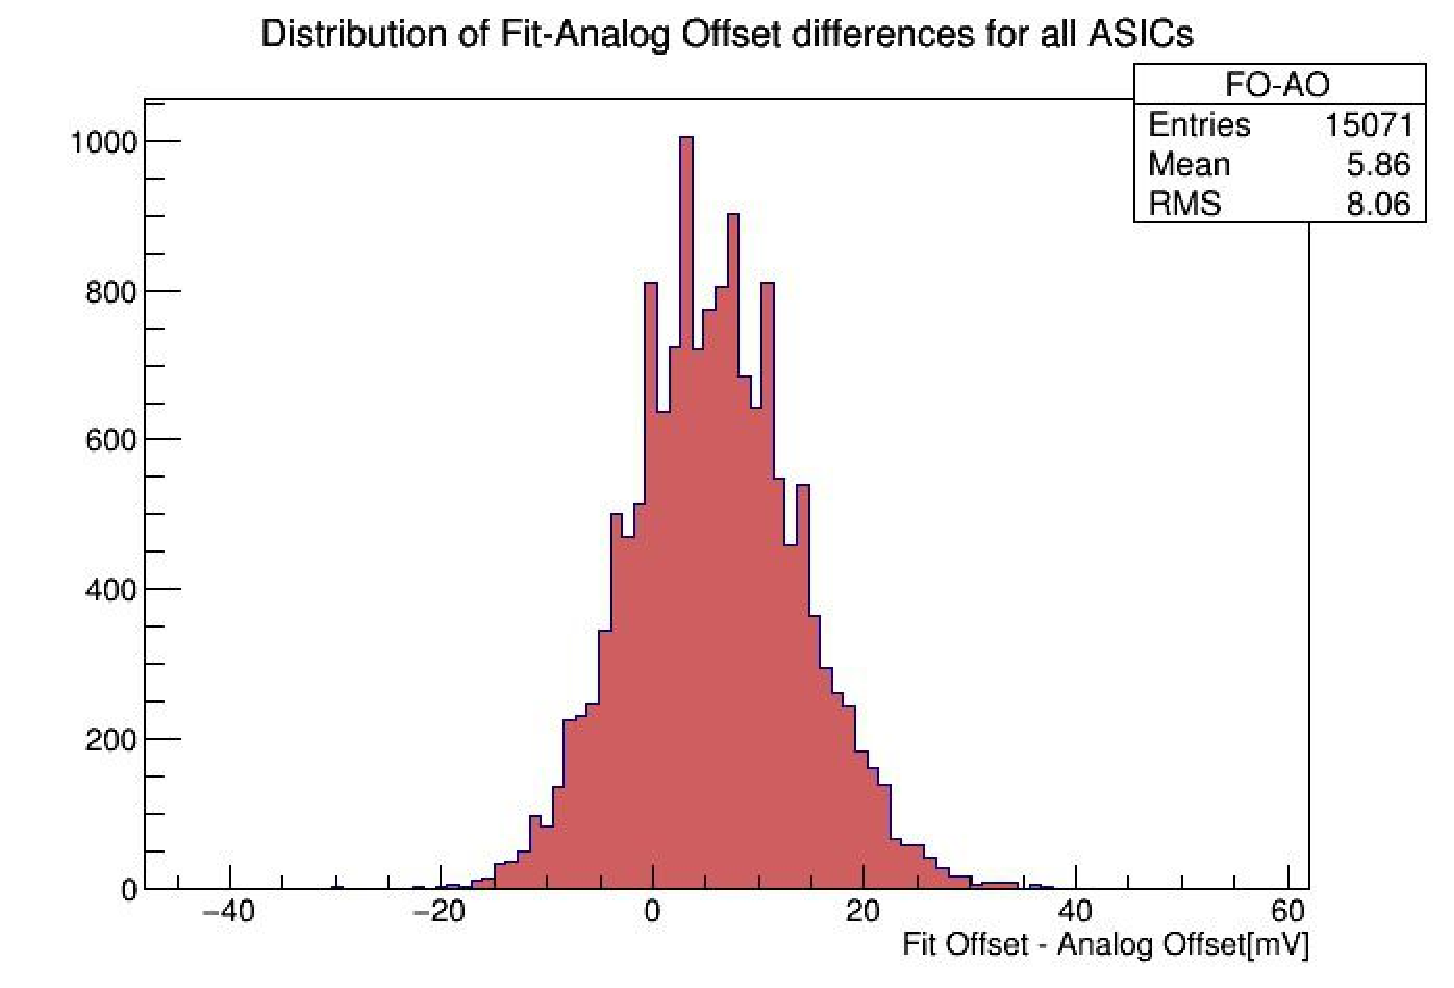
\includegraphics[width=\textwidth]{./Pictures/diffoffsetdif.pdf}
  \endminipage
  \caption{\textit{Left:} Distribution of offset calculated from the rate scan fitting. \textit{Right:} Distribution of the difference between the analog offset and the fit offset.}
  \label{fig:fitoffdist}
\end{figure}
Checking the correlation between the two offset values (fig~\ref{fig:offsetcor}) it can be observed that even there is a clear correlation between them, the fit offset is underestimating the analog offset measured.
In figure~\ref{fig:offch} the averaged offsets to all \glspl{asic}, separated by channels and adders are plotted. In general the offset takes similar values for all the channels and adders, without any remarkable outlier.
In table \ref{tab:allasicsdata} the average offsets to all \glspl{asic} in every single path are shown.

\begin{figure}
  \centering
  \minipage{0.5\textwidth}
  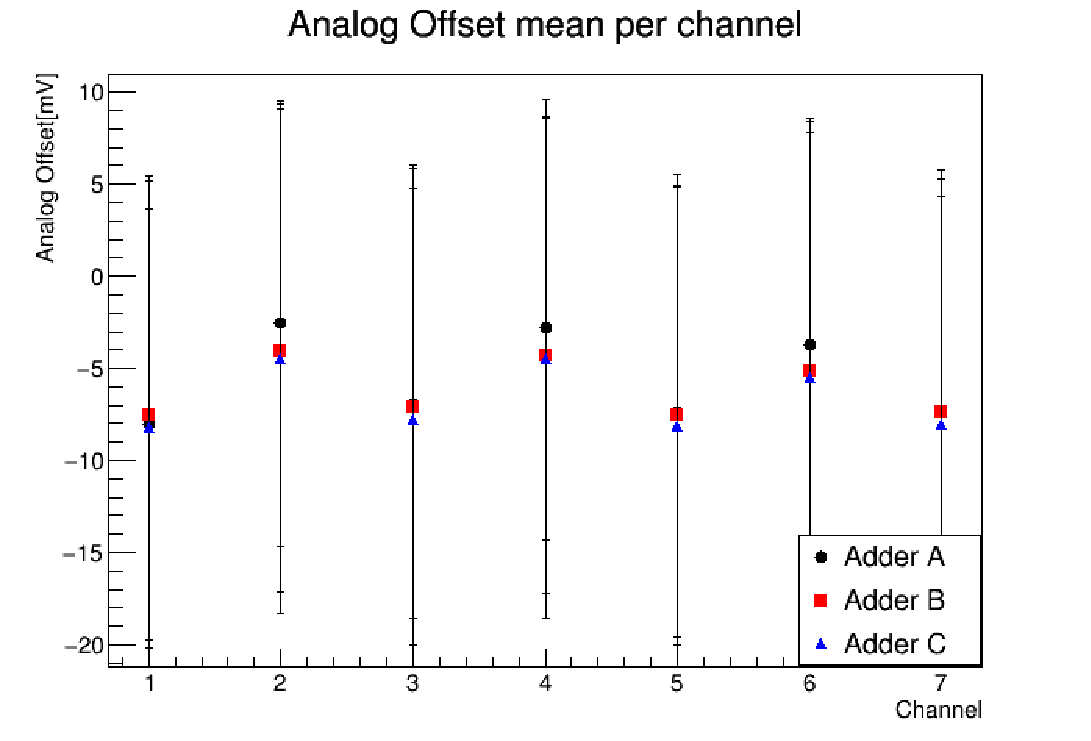
\includegraphics[width=\textwidth]{./Pictures/analogch.pdf}
  \endminipage
  \minipage{0.5\textwidth}
  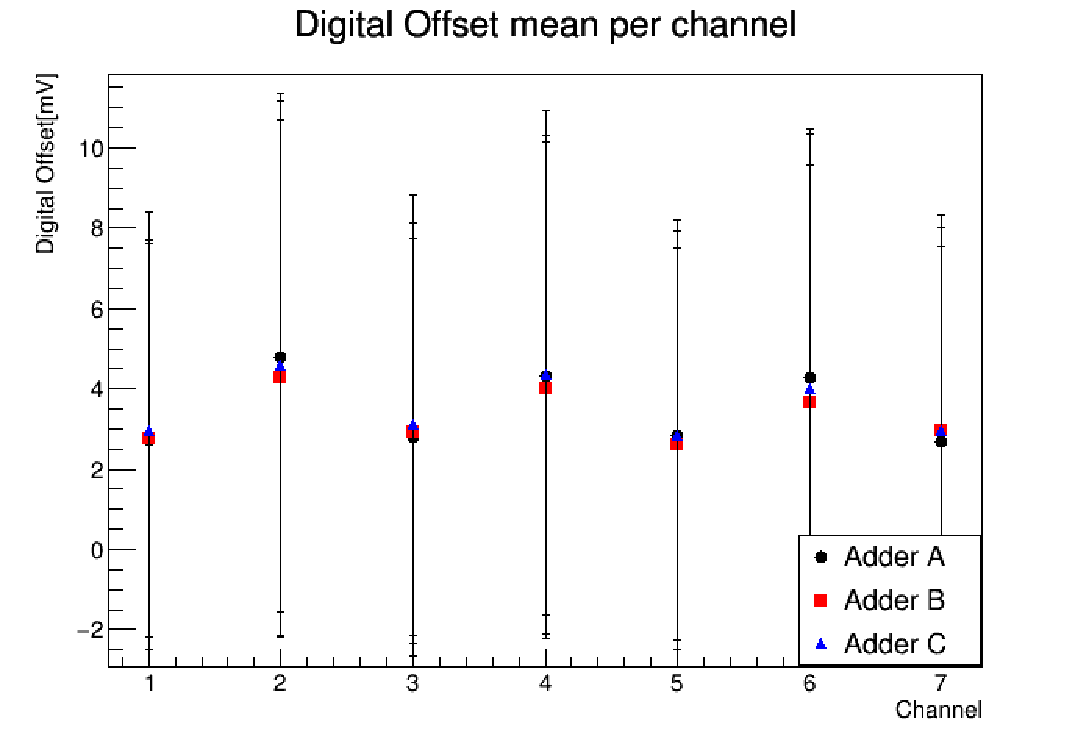
\includegraphics[width=\textwidth]{./Pictures/digitalch.pdf}
  \endminipage
  \caption{\textit{Left:} Analog offset averaged to all \glspl{asic} separated by channel and adder. \textit{Right:} Digital offset averaged to all \glspl{asic} separated by channel and adder.}
  \label{fig:offch}
\end{figure}

To find out which part of the \gls{asic} is responsible of the offset, correlation plots between channels, adders and discriminators were studied. Channels and discriminators show a clear correlation between pairs of them, but for adders, a real correlation is not observed. This implies that the offset do not depend on the channels or discriminators, but it is introduced by the adders. This result was expected from the original specifications of the \gls{asic}.

\subsection{Noise}

The noise in the \gls{asic} was measured during the Digital Offset test described in section~\ref{sec:digoff}. The noise again can only be measured when the output status is tagged as ``Pos''. In figure~\ref{fig:noisedist} the total distribution of noise values is shown, having an average noise of $5.186$ mV with RMS of $2.878$ mV. Several outliers were spotted and are marked in the plot, with noises very deviated from the mean. If we fit a gaussian profile to the distribution, the probability of having an outlier with noise over 40 mV is ~0\% and over 10 mV is less than 1\%. These outliers have been excluded
from the general characterization.
\begin{figure}[h]
  \centering
  \minipage{0.5\textwidth}
  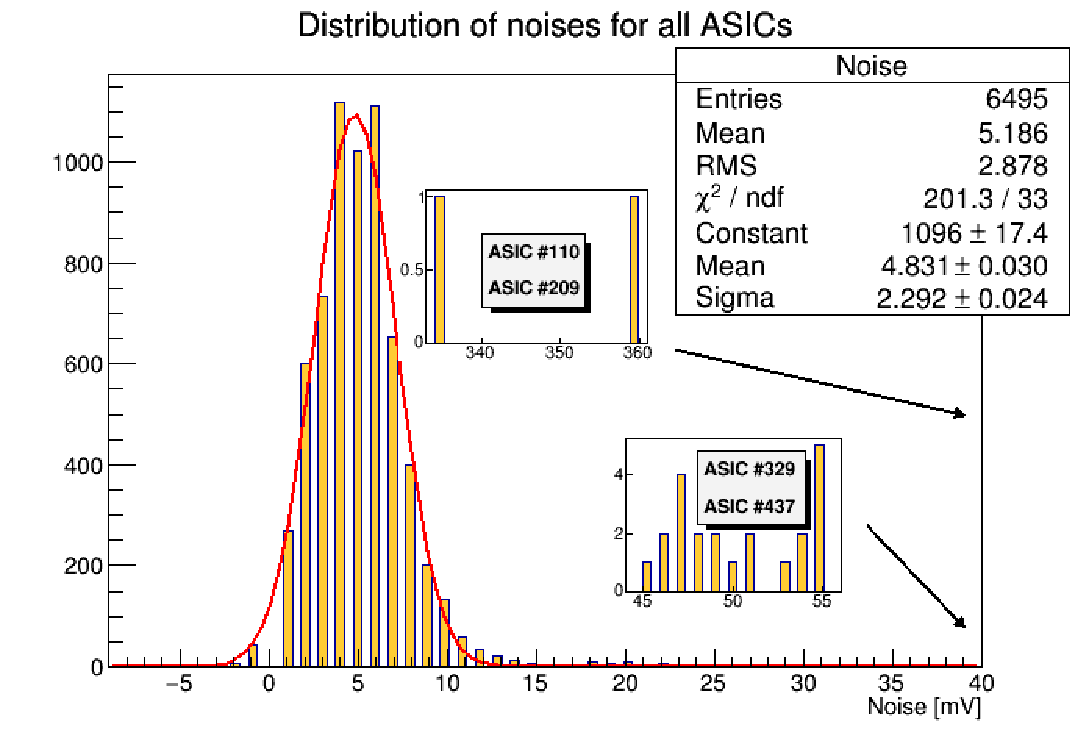
\includegraphics[width=\textwidth]{./Pictures/noisedist.pdf}
  \endminipage
  \minipage{0.5\textwidth}
  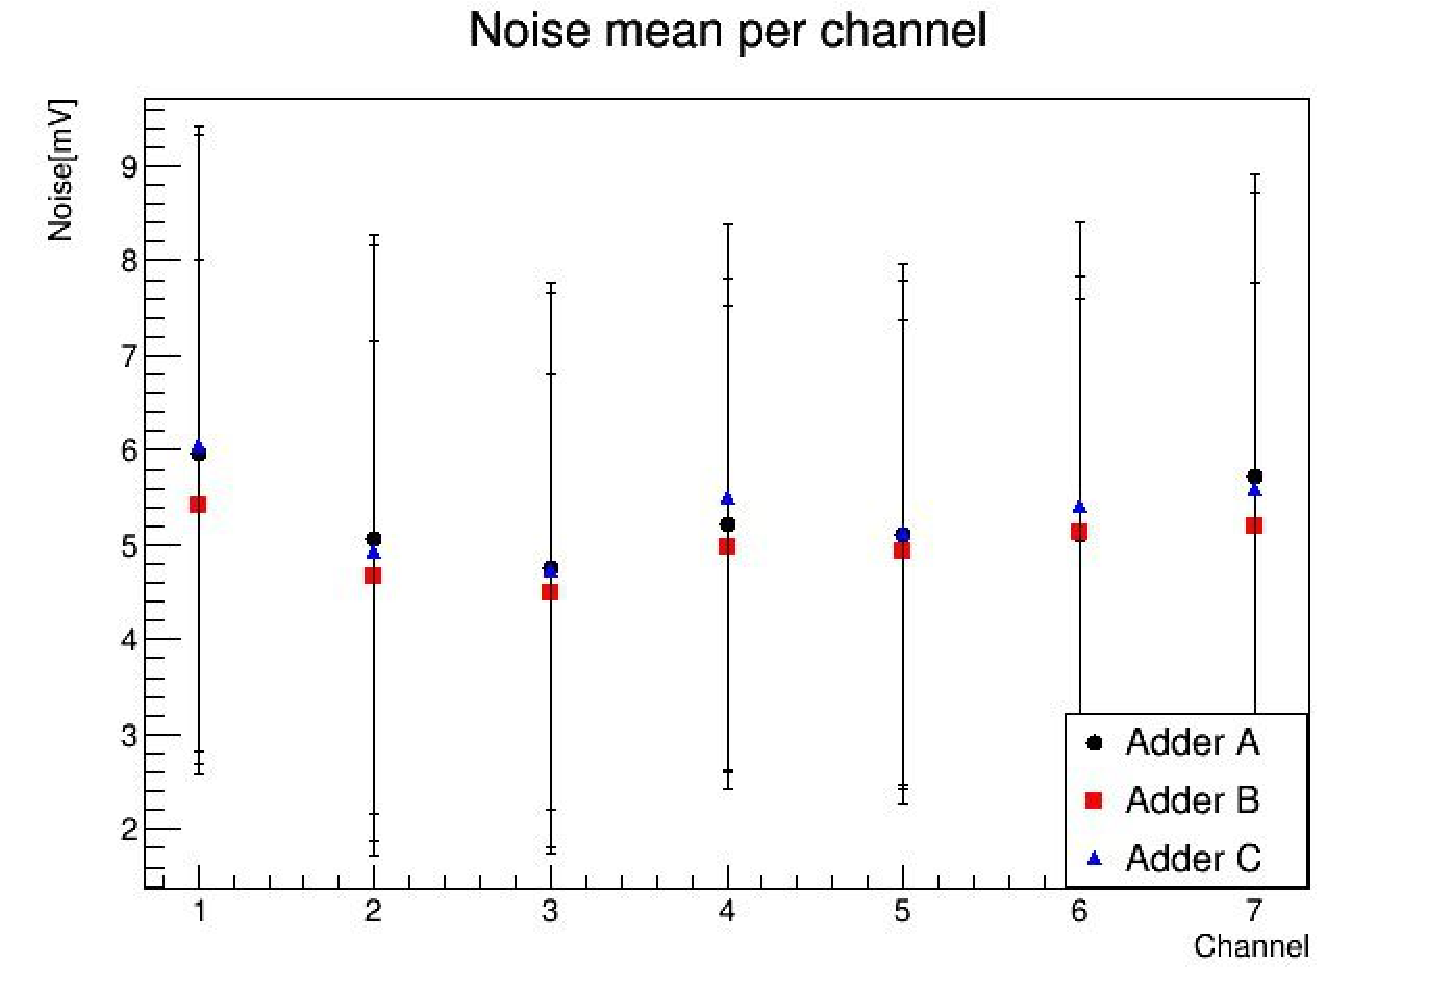
\includegraphics[width=\textwidth]{./Pictures/noisech.pdf}
  \endminipage
  \caption{\textit{Left:} Distribution of noises measured for all \glspl{asic}. Each entry represent the noise in a certain path (channel-adder-discriminator combination). The zoom-ins show the outliers. \textit{Right:} Noise averaged to all \glspl{asic} separated by channel and adder.}
  \label{fig:noisedist}
\end{figure}

No correlation of the noise between pairs of channels, adders or discriminators have been observed, so the noise is being introduced in each part of the \gls{asic} in a similar way.\\
In figure~\ref{fig:noisedist} the average noise value separated by channels and adders show that its value is mostly uniform.

\section{Characterization: Summary and discussion}


The gain measured in the \gls{asic} has a typical value of about $0,87\pm0,038$, having two channels that slightly differ from the rest. Is the case of the channels ( 2 and 3), that for all \glspl{asic} seem to have a deviation from the general mean, this effect is explanable by the setup configuration of the rate scan test. There are two \glspl{asic} where gain has a very low value, under 0,7, in several of their channels. Relative to the correlation study, there is not a strong correlation for the gain in any part of the \glspl{asic}, having all of them a correlation coefficient below 0,5.\\
The analog offsets measured in the test have a negative mean value, while the digital offset, as the rate scan only can provide possitive offsets, gives a positive mean value. In the correlation plots for the analog offset, it can be observed a positive correlation between channels, with correlation coefficients $\sim$0,8. For the adders however, no significant correlation is observed, concluding that in the adders, the offset measured is independent from each other, so they are the part of the \gls{asic} where the offset is introduced.
In the case of the digital offset, no correlation is observed at all, with coefficients very close to 0. It is needed to take into account that the data of digital offset is biased by the rate scan conditions.
From the correlation plot of digital and analog offset, we can say that both offsets have a correspondence and we are measuring the same feature, having a linear correlation with slope $\sim$1.
In summary, the offset expected from a typical \gls{asic} would be of $-6 \pm 13$ mV.\\
A method to calculate the offset of the \gls{asic} in an indirect way was applied assuming a model where the input signal and the rate scan result have a linear relation. The offset calculated by this method have in average, a difference with the analog offset of $5,86 \pm 8$ mV.
The correlation between the fit offset and the analog offset showed that they have a linear correlation by a factor of $0,774$.
The study of the fit offset in the different parts of the \glspl{asic} supported the idea that the adders are responsible for introducing the offset in the \gls{asic}.\\
Finally, in table \ref{tab:allasicsdata} are presented the values of gain, offset and noise, averaged to all the \glspl{asic} studied. This values represent the typical values that should be expected from a correctly functional \gls{asic}. If deviations from this numbers are observed, it might point to a defect in the \gls{asic}, meaning a bad performance that will not fit the specifications.

\begin{table}
  \centering
  \resizebox{\textwidth}{!}{%
    \begin{tabular}{llllllllllllll}
      \hline
      Disc. & Ch. & Add. & Gain & RMS & Analog & RMS[mV] & Digital & RMS[mV] & Fit & RMS[mV]& Noise[mV]& RMS[mV] \\
       &  &  &  &  &  Offset[mV] &  & Offset[mV] &  &  Offset[mV] & & & \\
      \hline
      0 & 1 & 0 &   0.870941 & 0.0347202 & -8.04178 & 11.7013 & 7.6831 & 5.41629 & 0.237361 & 12.2547 & 5.86861 & 3.00563 \\
      0 & 1 & 1 &   0.865733 & 0.0354431 & -2.56825 & 12.0754 & 9.26942 & 6.00255 & 5.42159 & 13.151 & 4.73869 & 2.65657 \\
      0 & 1 & 2 &   0.861889 & 0.0372319 & -6.90529 & 11.6572 & 7.38961 & 5.61574 & 0.459297 & 13.2761 & 4.40559 & 2.48136 \\
      0 & 2 & 0 &   0.838466 & 0.035875 & -2.82682 & 11.5199 & 8.88718 & 5.92886 & 4.81186 & 12.0241 & 5.08421 & 2.35825 \\
      0 & 2 & 1 &   0.833886 & 0.0374605 & -7.35196 & 12.2333 & 7.90845 & 5.88134 & 0.506872 & 13.5916 & 5 & 2.55973 \\
      0 & 2 & 2 &   0.830387 & 0.0369065 & -3.70752 & 12.1045 & 8.92932 & 6.18108 & 3.99229 & 12.8837 & 4.79679 & 2.44105 \\
      0 & 3 & 0 &   0.879369 & 0.0367518 & -7.35933 & 11.7325 & 7.87132 & 5.64872 & 0.784061 & 13.1786 & 5.64662 & 3.484 \\
      0 & 3 & 1 &   0.872314 & 0.0381587 & -7.52089 & 12.7001 & 7.58562 & 5.68263 & -0.450728 & 13.1254 & 5.22917 & 2.54056 \\
      0 & 3 & 2 &   0.871234 & 0.0377928 & -4.04735 & 13.1041 & 9.25946 & 6.80006 & 3.55013 & 14.3746 & 4.32 & 2.18838 \\
      0 & 4 & 0 &   0.869755 & 0.0373787 & -7.07521 & 12.9157 & 8.36331 & 6.00024 & 0.205656 & 13.5603 & 4.19231 & 2.25012 \\
      0 & 4 & 1 &   0.867655 & 0.0359559 & -4.30168 & 12.8884 & 8.9435 & 6.38963 & 2.65292 & 13.278 & 4.65497 & 2.18266 \\
      0 & 4 & 2 &   0.861649 & 0.0354134 & -7.55153 & 12.4649 & 7.70956 & 5.78174 & 0.0951152 & 13.1499 & 4.81395 & 2.60223 \\
      0 & 5 & 0 &   0.873273 & 0.0374989 & -5.17827 & 12.9837 & 8.79697 & 6.41468 & 1.78835 & 13.7437 & 4.80921 & 2.19069 \\
      0 & 5 & 1 &   0.870116 & 0.0359688 & -7.37604 & 12.6522 & 8.36525 & 5.49044 & -0.487576 & 13.7508 & 5.05839 & 2.46957 \\
      0 & 5 & 2 &   0.868586 & 0.0368392 & -8.2312 & 13.7086 & 8.84926 & 6.51816 & -0.999143 & 14.8268 & 5.9771 & 3.5693 \\
      0 & 6 & 0 &   0.86892 & 0.0393618 & -4.48189 & 13.8268 & 9.7963 & 7.14917 & 3.15424 & 15.5242 & 4.8895 & 3.11456 \\
      0 & 6 & 1 &   0.869291 & 0.0343526 & -7.76602 & 13.8442 & 8.83929 & 6.63897 & -0.61611 & 14.7812 & 4.48462 & 2.61721 \\
      0 & 6 & 2 &   0.866015 & 0.0360581 & -4.48324 & 14.1144 & 9.44624 & 6.93439 & 3.11168 & 14.9143 & 5.3587 & 2.9565 \\
      0 & 7 & 0 &   0.873033 & 0.0379731 & -8.15042 & 13.6576 & 8.28777 & 6.33279 & -0.973436 & 14.9387 & 4.92537 & 2.75526 \\
      0 & 7 & 1 &   0.872879 & 0.0360707 & -5.50418 & 14.0574 & 9.41124 & 7.01801 & 1.49357 & 14.6893 & 5.28402 & 3.06379 \\
      0 & 7 & 2 &   0.869562 & 0.0386874 & -8.07242 & 13.8974 & 8.32168 & 6.35307 & -0.732647 & 14.9372 & 5.6383 & 2.63978 \\
      1 & 1 & 0 &   0.881697 & 0.0341451 & -8.04178 & 11.7013 & 7.4927 & 5.56054 & -3.03256 & 12.605 & 6.04444 & 3.70158 \\
      1 & 1 & 1 &   0.876093 & 0.0328864 & -2.56825 & 12.0754 & 9 & 6.24797 & 2.56555 & 12.6045 & 5.40816 & 3.62626 \\
      1 & 1 & 2 &   0.872108 & 0.0318161 & -6.90529 & 11.6572 & 7.15753 & 5.46745 & -2.59383 & 12.1416 & 5.12057 & 3.43424 \\
      1 & 2 & 0 &   0.847899 & 0.0314701 & -2.82682 & 11.5199 & 8.46073 & 5.71851 & 1.5189 & 11.4802 & 5.34737 & 2.79574 \\
      1 & 2 & 1 &   0.845232 & 0.0323591 & -7.34819 & 12.2164 & 7.43103 & 5.58897 & -3.17824 & 13.3383 & 5.1958 & 2.79425 \\
      1 & 2 & 2 &   0.838856 & 0.0329706 & -3.70752 & 12.1045 & 8.5582 & 5.93878 & 0.9006 & 12.3124 & 5.41711 & 2.95009 \\
      1 & 3 & 0 &   0.890874 & 0.0358411 & -7.35933 & 11.7325 & 7.37132 & 5.31715 & -3.06684 & 12.7281 & 5.78195 & 2.88199 \\
      1 & 3 & 1 &   0.884409 & 0.0339822 & -7.52089 & 12.7001 & 7.07483 & 5.47237 & -3.13453 & 13.5406 & 5.6069 & 2.64522 \\
      1 & 3 & 2 &   0.883612 & 0.0325719 & -4.04735 & 13.1041 & 8.89503 & 6.50563 & 0.259641 & 13.9549 & 5.01156 & 2.73066 \\
      1 & 4 & 0 &   0.882881 & 0.034909 & -7.07521 & 12.9157 & 7.51034 & 5.7519 & -2.88689 & 13.3739 & 4.77698 & 2.30121 \\
      1 & 4 & 1 &   0.878196 & 0.0336269 & -4.30168 & 12.8884 & 8.66384 & 6.19265 & -0.0876289 & 13.5648 & 5.28977 & 2.82262 \\
      1 & 4 & 2 &   0.875941 & 0.0309881 & -7.55153 & 12.4649 & 7.20438 & 5.55088 & -3.23393 & 13.001 & 5.03759 & 2.28893 \\
      1 & 5 & 0 &   0.887686 & 0.034171 & -5.17827 & 12.9837 & 8.5122 & 6.00304 & -0.83976 & 12.6118 & 5.41718 & 2.66956 \\
      1 & 5 & 1 &   0.881864 & 0.0329572 & -7.37604 & 12.6522 & 7.61986 & 5.27637 & -3.32048 & 12.9181 & 5.34028 & 2.65666 \\
      1 & 5 & 2 &   0.877262 & 0.0327925 & -8.2312 & 13.7086 & 7.81071 & 5.98285 & -3.39332 & 14.0924 & 6.13971 & 3.1557 \\
      1 & 6 & 0 &   0.880771 & 0.0354957 & -4.48189 & 13.8268 & 9.3288 & 6.61699 & 0.871464 & 14.3059 & 4.99444 & 3.31913 \\
      1 & 6 & 1 &   0.878608 & 0.0332089 & -7.76602 & 13.8442 & 8.63603 & 6.52525 & -3.29734 & 13.35 & 4.96296 & 3.16791 \\
      1 & 6 & 2 &   0.87653 & 0.031666 & -4.48324 & 14.1144 & 9.18362 & 6.59579 & -0.118557 & 13.5596 & 5.63793 & 2.83065 \\
      1 & 7 & 0 &   0.887339 & 0.0345601 & -8.15042 & 13.6576 & 7.87037 & 6.10918 & -3.0437 & 13.7544 & 5.31579 & 2.9389 \\
      1 & 7 & 1 &   0.88383 & 0.033284 & -5.50418 & 14.0574 & 8.97059 & 6.77424 & -0.674379 & 13.6534 & 5.5503 & 2.8985 \\
      1 & 7 & 2 &   0.881967 & 0.0317656 & -8.07242 & 13.8974 & 7.93478 & 5.91143 & -3.7892 & 14.0832 & 5.56115 & 3.54846 \\
\hline

  \end{tabular}}
  \caption{Values of the gain, offset (measured by three different methods) and noise for the different parts of the typical ASIC, obtained averaging to all the ASICs tested.}
  \label{tab:allasicsdata}
\end{table}
\end{document}
